\documentclass[11pt,reqno]{amsart}

\usepackage[margin=0.95in]{geometry}
\usepackage{amsmath,amssymb,amsthm}
\usepackage{booktabs}
\usepackage{tabularx}
\usepackage{array}
\usepackage{xcolor}
\usepackage{tikz}
\usetikzlibrary{arrows.meta,positioning,fit,backgrounds}
\usepackage{enumitem}
\usepackage{microtype}
\usepackage{placeins}
\PassOptionsToPackage{obeyspaces}{url}
\usepackage{xurl}
\usepackage[hidelinks,colorlinks=true,linkcolor=blue!60!black,citecolor=teal!70!black,urlcolor=blue!70!black]{hyperref}

\theoremstyle{definition}
\newtheorem{definition}{Definition}[section]
\newtheorem{invariant}{Invariant}[section]
\newtheorem{remark}{Remark}[section]

\newcolumntype{Y}{>{\raggedright\arraybackslash}X}
\newcolumntype{P}[1]{>{\raggedright\arraybackslash}p{#1}}
\newcommand{\code}[1]{{\footnotesize\nolinkurl{#1}}}
\newcommand{\tcode}[1]{{\scriptsize\nolinkurl{#1}}}
\newcommand{\tagpa}{\textsc{program-audited}}
\newcommand{\tagem}{\textsc{empirical}}
\newcommand{\tagio}{\textsc{indicator-only}}
\newcommand{\tagul}{\textsc{upstream-linked}}
\newcommand{\tagoc}{\textsc{open-conj.}}

\title[OMEGA 4-Tier Multi-Scale Observatory (v6.7.0)]{OMEGA 4-Tier Multi-Scale Observatory (v6.7.0): Architecture, Render-Only Observer Isolation, Loopback Reverse-Proxy Telemetry, and Automated Verification Across Eight Local Artificial-Life Endpoints}

\author{Alexander Stephen Donahue}
\address{Independent Researcher, Spokane, WA, USA}
\email{0\_0@0thernes.art}
\urladdr{https://orcid.org/0009-0006-8168-9648}

\date{November 25, 2026}
\subjclass[2020]{Primary 68U20, 68N30; Secondary 92C15, 68M14}
\keywords{multi-scale observatory, artificial life, observer independence, reverse proxy, WebGL2, telemetry metrology, mutation testing, property-based testing}

\begin{document}

\begin{abstract}
Multi-scale Artificial Life research pipelines spanning molecular replicators, cellular embryogenesis, embodied neural ecosystems, and planetary habitats rarely expose synchronized telemetry without either contaminating simulation state with observer side effects or collapsing heterogeneous interfaces into brittle monolithic scripts. We present Version~6.7.0 of the \emph{OMEGA 4-Tier Multi-Scale Observatory} (\code{omega-triscale-observatory}), a zero-dependency Node.js~ESM, Python~3, and WebGL~2.0 local orchestration, reverse-proxy, and metrology cockpit supervising eight local endpoints across seven public repositories on \code{127.0.0.1:8790}. The hub aggregates Server-Sent Events (SSE), binary \code{AZST} snapshots, WebSocket streams, and HTTP control surfaces spanning Tier~1 molecular genomes (\code{AUTOPHAGE}, \code{:8787}), Tier~2 cellular embryogenesis (\code{Cellulogonic Mecha}, \code{:8788}), Tier~2+ frontier virtual-cell testbeds (\code{Cellular Engine Omega}, \code{:8791}), Tier~3/4 cognitive verification (\code{Noetic Organism Omega}, \code{:8795}), dual Tier~3+4 ecosystem worlds (\code{Asmodensius-Native} WebGL2 \code{:8794} and native \code{az\_view} \code{:8796}), the unified cockpit (\code{:8790}), and the offline \code{Zeta-Omega} singularity atlas (\code{:8790/zeta-omega/}).

Architecturally, the observatory enforces four auditable engineering guarantees: (i) a strict render-only observer boundary (\code{D7RO}) preventing live T1/T2 state writes into \code{Asmodensius-Native} while preserving shader \code{\#ifdef PICK} hit-testing; (ii) a fail-closed loopback HTTP/WebSocket CSRF/CSWSH and path-traversal security perimeter; (iii) bounded bare-metal Windows launch controls ($1$--$1{,}000{,}000$ founders, $23$-bit lesion bitmask, \code{AVX2/VNNI}, \code{24C P+E}, \code{DDR5} prefetch, \code{RTX 5070 Ti CUDA PTX}, large pages) differentially verified between Node and Python; and (iv) a deterministic 112-trait spectral differential, 8-axis biophysical cosine coherence, and rolling $\le 240$-sample omnitemporal ring buffer. Automated verification passes $12/12$ Node integration/property/metamorphic tests ($250$ seeded \code{prop\_check} trials), $5/5$ Python relay tests ($120$ seeded trials), static lint hygiene, and $6/6$ ($100.0\%$) surgical mutation kills.

\emph{Honest epistemic and peer-review boundary:} This technical architecture preprint has not undergone formal external peer review. The observatory is strictly a visualization, telemetry, and process-orchestration instrument; it contains $0$ local Lean~4 proof files (upstream formal proofs live in six formal sibling repositories) and retires zero ($0 / 1{,}900$) overarching open problems in the \emph{Unsolved Problems Mega-Atlas}.
\end{abstract}

\maketitle

\section{Introduction and Scope}
\label{sec:intro}

Long-running Artificial Life investigations frequently confront an instrumentation dilemma: open-ended evolutionary dynamics~\cite{bedau1998,taylor2016}, autopoietic boundary maintenance~\cite{varela1974}, and multi-scale developmental coordination~\cite{levin2022} unfold simultaneously across molecular, cellular, organismal, and environmental scales, yet ad-hoc inspection hooks easily perturb simulation random-number streams, corrupt conservation ledgers, or expose insecure local administrative endpoints to cross-origin browser requests. Moreover, when independent engines are developed across heterogeneous native toolchains (C11, freestanding C23, CUDA PTX, x86-64 JIT, and Lean~4~\cite{moura2021}), researchers require a clean, reproducible supervisory plane that observes and couples explicitly permitted channels without silently violating engine isolation laws.

\emph{OMEGA 4-Tier Multi-Scale Observatory} v6.7.0 addresses this engineering problem as a lightweight, zero-npm-dependency, zero-pip-dependency local supervisor. By extracting all security predicates, Genesis configuration normalizers, binary \code{AZST} decoders, 112-trait spectral differentials, and \code{D7RO} coupling-matrix invariants into a pure ES module (\code{lib/observatory\_core.mjs}) paired with a dry-run-testable Python relay (\code{macro\_wild\_relay.py}), the instrument achieves full cross-platform automated verification, differential Node--Python parity, and $100\%$ surgical mutation coverage without requiring external proprietary services or leaving background daemons running after tests.

\section{Numbered Claims Ledger}
\label{sec:claims}

Every headline engineering and empirical claim made by this repository is indexed in Table~\ref{tab:claims} with an explicit epistemic tier tag, primary reproducible artifact, and falsification condition (full command ledger in \code{CLAIMS.md}).

\begin{table}[t]
\centering
\caption{Numbered Claims Ledger for \code{omega-triscale-observatory} v6.7.0 separating program-audited runtime invariants from empirical latency measurements, indicator-only heuristics, upstream links, and open conjectures.}
\label{tab:claims}
\scriptsize
\renewcommand{\arraystretch}{1.18}
\begin{tabularx}{\textwidth}{@{}P{0.48cm}P{2.05cm}YP{2.75cm}P{2.55cm}@{}}
\toprule
\textbf{ID} & \textbf{Tier} & \textbf{Exact Claim Statement} & \textbf{Primary Artifact} & \textbf{Refutation Condition} \\
\midrule
C1 & \tagpa & Loopback perimeter enforces \code{127.0.0.1}/\code{localhost}/\code{[::1]} Host/Origin, \code{application/json} POST, \code{Sec-Fetch-Site}, and \code{resolveSafePath} traversal defense. & \tcode{lib/observatory_core.mjs}, \tcode{tests/test_observatory.mjs} & Any cross-origin POST/SSE or traversal succeeds ($200$). \\
C2 & \tagpa & Genesis normalizer clamps $n \in [1, 10^6]$, $\mathrm{cap} \in [n, 2{\times}10^6]$, $\mathrm{species} \in [1, \min(100, n)]$, $23$-bit lesion mask, and matches Python \tcode{--dry-run}. & \tcode{lib/observatory_core.mjs}, \tcode{macro_wild_relay.py} & Any \tcode{prop\_check} trial or Node--Python parity mismatch. \\
C3 & \tagpa & Render-only observer boundary keeps \tcode{matrix4x4} T1/T2$\to$T3/T4 strictly \tcode{D7RO} ($s=0$) and preserves \tcode{\#ifdef PICK} in WebGL2 Bio-FX injection. & \tcode{lib/observatory_core.mjs}, \tcode{server.mjs} & Any T1/T2 write to T3/T4 or altered \tcode{\#ifdef PICK}. \\
C4 & \tagpa & 112-trait spectral delta clamps inputs to $[0,1]$, satisfies swap antisymmetry and shift invariance, and caps omnitemporal history $\le 240$. & \tcode{computeDifferentialsCore}, \tcode{tests/test_observatory.mjs} & History $> 240$, NaN output, or symmetry violation. \\
C5 & \tagpa & Conservation gate fails closed (\tcode{ALERT} on any residual or \tcode{observerFail} $\neq 0$; \tcode{DEGRADED} on stale/offline tiers; never false-green). & \tcode{computeDifferentialsCore}, \tcode{server.mjs} & Reports \tcode{VERIFIED} when offline or residual $\neq 0$. \\
C6 & \tagpa & Automated suite passes $12/12$ Node tests ($250$ \tcode{prop\_check}), $5/5$ Python tests ($120$ trials), static lint, and $6/6$ ($100\%$) surgical mutants killed. & \tcode{scripts/run_mutation_audit.mjs}, \tcode{results/mutation_audit.json} & Any test failure or surviving planted mutant. \\
C7 & \tagem & Measured local Node~v25.8.2 latency averages $0.0804\text{ ms}$ for differentials and $4.5210\text{ ms}$ for $10{,}000$-creature binary \tcode{AZST} decoding. & \tcode{scripts/benchmark_observatory.mjs}, \tcode{results/benchmarks.json} & Re-run on reference host diverges outside variance. \\
C8 & \tagio & Volatility index \tcode{chaosLyapunov} and count-driven T3 organ meshes are heuristic visualization indicators, not Lyapunov exponents or anatomical coordinates. & \tcode{LIMITATIONS.md}, \tcode{web/creature_gl.js} & Claiming physical/Lyapunov equivalence without proof. \\
C9 & \tagul & Repo contains $0$ local Lean~4 files; six formal sibling repos report $327$ combined upstream 6-kernel Lean~4.35.0 theorems audited in their own repos. & \tcode{README.md}, \tcode{docs/MEGA_ATLAS_CROSSCHECK.md} & Upstream repo audit count changes without sync. \\
C10 & \tagoc & Zero ($0 / 1{,}900$) overarching Mega-Atlas open problems (\tcode{AI-045}, \tcode{SYS-009}, \tcode{SYS-050}) are solved or retired by this instrument. & \tcode{docs/MEGA_ATLAS_CROSSCHECK.md} & Peer-reviewed resolution of a parent Atlas ID. \\
\bottomrule
\end{tabularx}
\end{table}

\section{Four-Tier Eight-Endpoint Architecture}
\label{sec:architecture}

Figure~\ref{fig:arch} illustrates the topology of the observatory. A single loopback HTTP/1.1~\cite{rfc9110} and WebSocket~\cite{rfc6455} supervisor (\code{server.mjs} on \code{127.0.0.1:8790}) manages lifecycle supervision, reverse-proxy URL rewriting, binary telemetry decoding, Server-Sent Events (SSE)~\cite{htmlsse} broadcasting, and WebGL~2.0~\cite{webgl2spec} client rendering across eight endpoints spanning seven public repositories (Table~\ref{tab:endpoints}).

\begin{figure}[t]
\centering
\resizebox{\textwidth}{!}{%
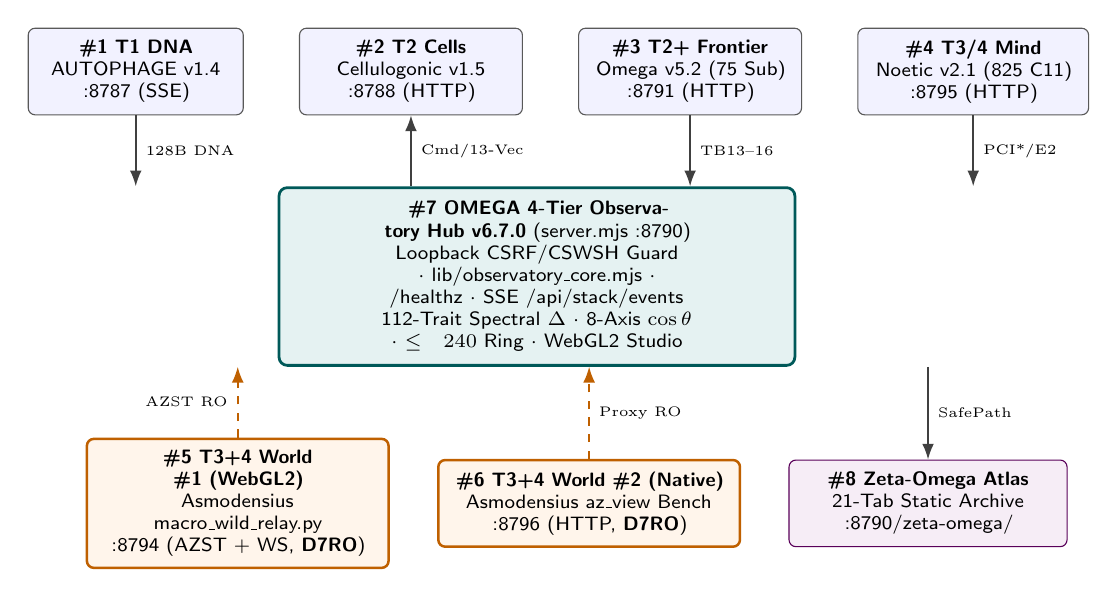
\begin{tikzpicture}[
  font=\sffamily\scriptsize,
  node distance=6mm and 7mm,
  box/.style={draw=black!65, rounded corners=2.5pt, align=center, inner sep=4pt, minimum height=11mm, fill=blue!5},
  hub/.style={draw=teal!70!black, line width=1pt, rounded corners=3pt, align=center, inner sep=5pt, minimum height=13mm, fill=teal!10},
  robox/.style={draw=orange!75!black, line width=0.9pt, rounded corners=2.5pt, align=center, inner sep=4pt, minimum height=11mm, fill=orange!8},
  atlas/.style={draw=violet!70!black, rounded corners=2.5pt, align=center, inner sep=4pt, minimum height=11mm, fill=violet!7},
  arr/.style={-{Latex[length=2mm]}, semithick, draw=black!75},
  darr/.style={-{Latex[length=2mm]}, semithick, dashed, draw=orange!75!black}
]
  \node[box, text width=2.45cm] (t1) {\textbf{\#1 T1 DNA}\\AUTOPHAGE v1.4\\\tcode{:8787} (SSE)};
  \node[box, right=of t1, text width=2.55cm] (t2) {\textbf{\#2 T2 Cells}\\Cellulogonic v1.5\\\tcode{:8788} (HTTP)};
  \node[box, right=of t2, text width=2.55cm] (t2p) {\textbf{\#3 T2+ Frontier}\\Omega v5.2 (75 Sub)\\\tcode{:8791} (HTTP)};
  \node[box, right=of t2p, text width=2.65cm] (t3n) {\textbf{\#4 T3/4 Mind}\\Noetic v2.1 (825 C11)\\\tcode{:8795} (HTTP)};

  \node[hub, below=9mm of t2, xshift=16mm, text width=6.2cm] (hub) {\textbf{\#7 OMEGA 4-Tier Observatory Hub v6.7.0} (\tcode{server.mjs :8790})\\
    Loopback CSRF/CSWSH Guard $\cdot$ \tcode{lib/observatory\_core.mjs} $\cdot$ \tcode{/healthz} $\cdot$ SSE \tcode{/api/stack/events}\\
    112-Trait Spectral $\Delta$ $\cdot$ 8-Axis $\cos\theta$ $\cdot$ $\le 240$ Ring $\cdot$ WebGL2 Studio};

  \node[robox, below=9mm of hub, xshift=-38mm, text width=3.55cm] (w1) {\textbf{\#5 T3+4 World \#1 (WebGL2)}\\Asmodensius \tcode{macro\_wild\_relay.py}\\\tcode{:8794} (AZST + WS, \textbf{D7RO})};
  \node[robox, right=6mm of w1, text width=3.55cm] (w2) {\textbf{\#6 T3+4 World \#2 (Native)}\\Asmodensius \tcode{az\_view} Bench\\\tcode{:8796} (HTTP, \textbf{D7RO})};
  \node[atlas, right=6mm of w2, text width=3.25cm] (zeta) {\textbf{\#8 Zeta-Omega Atlas}\\21-Tab Static Archive\\\tcode{:8790/zeta-omega/}};

  \draw[arr] (t1) -- node[right, font=\tiny]{128B DNA} (hub.north -| t1);
  \draw[arr] (hub.north -| t2) -- node[right, font=\tiny]{Cmd/13-Vec} (t2);
  \draw[arr] (t2p) -- node[right, font=\tiny]{TB13--16} (hub.north -| t2p);
  \draw[arr] (t3n) -- node[right, font=\tiny]{PCI*/E2} (hub.north -| t3n);

  \draw[darr] (w1.north) -- node[left, font=\tiny]{AZST RO} (hub.south -| w1);
  \draw[darr] (w2.north) -- node[right, font=\tiny]{Proxy RO} (hub.south -| w2);
  \draw[arr] (hub.south -| zeta) -- node[right, font=\tiny]{SafePath} (zeta.north);
\end{tikzpicture}%
}
\caption{Four-tier, eight-endpoint architecture of \code{omega-triscale-observatory} v6.7.0. Solid arrows indicate loopback control/telemetry channels; dashed orange arrows denote the strict \code{D7RO} read-only observer boundary into \code{Asmodensius-Native} (zero live T1/T2 state writes during ticks).}
\label{fig:arch}
\end{figure}

\begin{table}[t]
\centering
\caption{All eight supervised local endpoints mapped to their scale tier, transport protocol, upstream repository, and observer write policy.}
\label{tab:endpoints}
\scriptsize
\setlength{\tabcolsep}{3.5pt}
\renewcommand{\arraystretch}{1.15}
\begin{tabularx}{\textwidth}{@{}P{0.4cm}P{1.55cm}P{2.35cm}YP{1.75cm}P{1.65cm}@{}}
\toprule
\textbf{\#} & \textbf{Tier} & \textbf{Local Endpoint} & \textbf{Supervised Instrument / Upstream Repo} & \textbf{Transport} & \textbf{Policy} \\
\midrule
1 & T1 ($10^{-9}\text{ m}$) & \tcode{127.0.0.1:8787} & \tcode{AUTOPHAGE v1.4.0} (\tcode{0thernes/autophage}) & HTTP + SSE & Read/Cmd \\
2 & T2 ($10^{-6}\text{ m}$) & \tcode{127.0.0.1:8788} & \tcode{Cellulogonic Mecha v1.5.0} (\tcode{cellulogonic-mecha}) & HTTP JSON & Read/Cmd \\
3 & T2+ & \tcode{127.0.0.1:8791} & \tcode{Cellular Engine Omega v5.2.0} (\tcode{cellular-engine-omega}) & HTTP JSON & Read/Poll \\
4 & T3/4 & \tcode{127.0.0.1:8795} & \tcode{Noetic Organism Omega v2.1.0} (\tcode{noetic-organism-omega}) & HTTP JSON & Read/DNA \\
5 & T3+4 W1 & \tcode{127.0.0.1:8794} & \tcode{Asmodensius-Native v1.1.0} WebGL2 (\tcode{asmodensius-native}) & AZST + WS & \textbf{D7RO} \\
6 & T3+4 W2 & \tcode{127.0.0.1:8796} & \tcode{Asmodensius-Native v1.1.0} \tcode{az\_view} (\tcode{asmodensius-native}) & HTTP Proxy & \textbf{D7RO} \\
7 & Hub & \tcode{127.0.0.1:8790} & \tcode{OMEGA Observatory v6.7.0} (this repository) & HTTP, SSE, WS & Supervisor \\
8 & Atlas & \tcode{:8790/zeta-omega/} & \tcode{Zeta-Omega v3.4.0} (\tcode{alife-singularity-omega-package}) & Static Safe & Read-Only \\
\bottomrule
\end{tabularx}
\end{table}

\subsection{Reverse Proxy, Security Perimeter, and Health Observability}
All browser traffic terminates at \code{127.0.0.1:8790}. The server enforces four defense-in-depth controls implemented in \code{lib/observatory\_core.mjs}:
\begin{enumerate}[leftmargin=1.5em,itemsep=2pt]
  \item \emph{Loopback Host/Origin/Fetch Guard} (\code{isSafeLoopbackRequest}): rejects non-loopback \code{Host} or \code{Origin} headers, blocks cross-site \code{Sec-Fetch-Site} values, requires \code{application/json} on \code{POST /api/stack/action}, and applies identical loopback verification on WebSocket \code{upgrade} handshakes (\code{/proxy/macro/ws}) to mitigate cross-site request forgery (CSRF) and cross-site WebSocket hijacking (CSWSH).
  \item \emph{Canonical Path Containment} (\code{resolveSafePath}): rejects NUL bytes (\code{\textbackslash 0}), drive-letter prefixes, UNC paths, backslash escapes, and \code{..} relative traversals via \code{path.relative} before serving static UI assets or \code{/zeta-omega/} archives.
  \item \emph{Strict Parameter Validation and Caps}: enforces non-negative integer parsing on \code{/api/stack/shape/:clade} and \code{/api/stack/env-slice?z=}, bounds proxy request bodies to $2\text{ MiB}$, proxy buffered rewrites to $16\text{ MiB}$, JSON action bodies to $256\text{ KiB}$, and concurrent SSE clients to $32$.
  \item \emph{Structured Health Endpoint}: exposes \code{GET /healthz} returning service version (\code{6.7.0}), uptime, engine connectivity booleans, conservation gate status, and active SSE subscriber count.
\end{enumerate}

\section{Render-Only Observer Independence and Telemetry Mathematics}
\label{sec:math}

A central architectural invariant of \code{Asmodensius-Native} is Law~4 / \code{D7} observer independence: observing or visualizing a running simulation must never alter simulation state or PRNG trajectories (e.g., counter-based Philox streams~\cite{salmon2011}). The observatory enforces this invariant at two independent layers:

\begin{invariant}[Zero-Observer-Interference \code{D7RO} Coupling Matrix]
\label{inv:d7ro}
Let $M \in (\mathcal{M} \times [0,1])^{4 \times 4}$ denote the coupling matrix emitted by \code{computeDifferentialsCore} across tiers $(T_1, T_2, T_3, T_4)$. For all operator toggle configurations (\code{autoCouple}, \code{envToCellsSolvent}, \code{reseedOnLock}, \code{waveMode}), every cross-tier entry from lower tiers $(T_1, T_2)$ into the \code{Asmodensius-Native} tiers $(T_3, T_4)$ satisfies
\begin{equation}
  M_{r,c} = (\mathrm{D7RO},\, 0) \qquad \forall (r, c) \in \{0, 1\} \times \{2, 3\}.
  \label{eq:d7ro}
\end{equation}
Furthermore, when proxy Bio-FX GLSL~ES~3.00 shaders are injected into \code{/proxy/macro/viewer\_gl.js}, vertex/fragment mutations apply strictly outside \code{\#ifdef PICK} blocks so GPU specimen picking remains bit-identical.
\end{invariant}

\subsection{112-Trait Spectral Differential and 8-Axis Cosine Coherence}
Given raw Tier~1 DNA traits $a \in \mathbb{R}^{112}$ and Tier~2 cellular traits $b \in \mathbb{R}^{112}$ (whose upstream slots may exceed $[0,1]$), we first clamp $\tilde{a}_i = \operatorname{clip}_{[0,1]}(a_i)$ and $\tilde{b}_i = \operatorname{clip}_{[0,1]}(b_i)$ and compute:
\begin{equation}
  \Delta_i = \tilde{b}_i - \tilde{a}_i \in [-1, 1], \qquad
  g_j = \Delta_{j+1} - \Delta_j \;\;(0 \le j < 111), \qquad
  |\bar{\Delta}| = \frac{1}{112}\sum_{i=0}^{111} |\Delta_i|.
  \label{eq:delta112}
\end{equation}
Because raw slot semantics differ across T1 and T2, cross-tier directional coherence is computed on a semantically aligned 8-axis normalized biophysical vector $u, v \in [0, 1]^8$ (vitality index, alive count, assembly index, distinct lineages, holobiont/tissue size, causal length/active loci, entropy/microtubule frequency, and log-backlash):
\begin{equation}
  \cos\theta(u, v) =
  \begin{cases}
    \dfrac{\langle u, v \rangle}{\|u\|_2 \, \|v\|_2} & \text{if } \|u\|_2^2 > 10^{-9} \text{ and } \|v\|_2^2 > 10^{-9}, \\[8pt]
    0 & \text{otherwise.}
  \end{cases}
  \label{eq:cos8}
\end{equation}
Population clade diversity and 24-bin hue diversity decoded from binary \code{AZST} creature snapshots use Shannon entropy $H = -\sum_{k: c_k > 0} (c_k / N) \log_2 (c_k / N)$~\cite{shannon1948}. Each differential tick appends one summary frame to a rolling omnitemporal ring buffer capped strictly at $L_{\max} = 240$ entries to guarantee $O(1)$ bounded memory growth.

\subsection{Fail-Closed Conservation Gate}
The top-bar conservation state transitions strictly across three values: \code{ALERT} whenever any Tier~1 ledger residual, Tier~2 mass/energy/second-law residual, or \code{observerFail} counter is nonzero; \code{VERIFIED} only if all three tiers (T1, T2, T4) are online with telemetry timestamps fresher than $15\text{ s}$ and zero residuals; and \code{DEGRADED} otherwise. Offline engines can never render a false-green \code{VERIFIED} badge.

\section{Bare-Metal Windows Control Surface and Relay Parity}
\label{sec:baremetal}

To support desktop stress exploration on hybrid-core Windows workstations (e.g., 24-core 8P+16E CPUs with DDR5 and NVIDIA RTX~5070~Ti GPUs), the Genesis Studio drawer and \code{macro\_wild\_relay.py} expose bounded hardware controls while preventing out-of-range crashes or command-argument injection:
\begin{itemize}[leftmargin=1.5em,itemsep=2pt]
  \item \emph{Population and Carrying Capacity}: founder count $n \in [1, 1{,}000{,}000]$ with quick step controls ($100$, $1\text{k}$, $10\text{k}$, $100\text{k}$, presets up to \code{million}); carrying capacity defaults to $\min(1{,}004{,}096,\, 4n + 4096)$ for $n \le 250{,}000$ and $\max(n + 4096,\, 1{,}004{,}096)$ above, clamped to $[n, 2{,}000{,}000]$.
  \item \emph{Species, Grid, and 23-Bit Lesion Mask}: founder species clamped to $[1, \min(100, n)]$ matching upstream \code{WG\_MAX\_SPECIES}; 3D log2 grid dimensions clamped to $[2, 8]^3$ or \code{auto}; 23 native behavior/cognition flags masked strictly by \code{0x7fffff}; arbitrary parameter keys whitelisted to \code{\^{}[A-Z0-9\_]+\$} with finite integer values.
  \item \emph{Hardware Execution Flags}: \code{--kernels \{0,1\}} (AVX2/AVX-VNNI vector paths), \code{--ecores} (all 24 P+E physical cores), \code{--prefetch \{0,1\}} (DDR5 software prefetch), \code{--gpu \{0,1\}} (CUDA PTX sparse brain offload), and \code{--large-pages} (2~MiB TLB huge pages).
\end{itemize}
Both \code{lib/observatory\_core.mjs} (Node) and \code{macro\_wild\_relay.py --dry-run} (Python) implement identical clamping semantics, verified differentially by our automated test suite.

\section{Automated Verification, Mutation Audit, and Benchmarks}
\label{sec:verification}

All verification runs execute cleanly with zero external npm/pip packages and zero lingering daemon processes (the live HTTP test suite binds \code{server.mjs} to ephemeral port \code{127.0.0.1:0} and closes it in \code{t.after()}):
\begin{itemize}[leftmargin=1.5em,itemsep=2pt]
  \item \textbf{Node~25 Built-In Test Suite (\code{tests/test\_observatory.mjs}):} $12/12$ PASS covering \code{node --check} + \code{py\_compile}, version/identity audit, Genesis clamping, hardware flags, path-traversal and CSRF/CSWSH rejection, live ephemeral HTTP contract tests (\code{/healthz}, static \code{nosniff}, traversal blocks, invalid \code{clade}/\code{z} returning \code{400}, CSRF \code{403}), $250$ deterministic seeded \code{prop\_check} randomized trials, metamorphic 112-trait swap/shift/clamp invariance, omnitemporal $\le 240$ cap, \code{D7RO} invariant, \code{\#ifdef PICK} preservation, binary \code{AZST} decoding, and Node--Python \code{--dry-run} differential parity.
  \item \textbf{Python Relay Test Suite (\code{tests/test\_relay.py}):} $5/5$ PASS including $120$ seeded randomized trials of \code{resolve\_relay\_options} and subprocess \code{--dry-run} CLI verification.
  \item \textbf{Static Lint Hygiene (\code{scripts/lint\_check.mjs}):} $9$ JS/MJS + $2$ Python targets, $0$ errors (rejects \code{eval}, \code{new Function}, \code{Math.random()} in core logic, and stale affiliation strings).
  \item \textbf{Surgical Mutation Testing (\code{scripts/run\_mutation\_audit.mjs}):} Following mutation-testing methodology~\cite{jia2011}, six logic regressions are planted inside an isolated temporary workspace copy and executed against the test suite; $6/6$ ($100.0\%$) mutants are killed (Table~\ref{tab:mutants}).
\end{itemize}

\begin{table}[t]
\centering
\caption{Surgical mutation audit results (\code{results/mutation\_audit.json}, $6/6 = 100.0\%$ kill rate) and deterministic telemetry micro-benchmarks (\code{results/benchmarks.json}, Node v25.8.2 on Windows~x64).}
\label{tab:mutants}
\scriptsize
\renewcommand{\arraystretch}{1.15}
\begin{tabularx}{\textwidth}{@{}P{3.65cm}YP{1.45cm}P{1.45cm}@{}}
\toprule
\textbf{Planted Mutant ID} & \textbf{Injected Logic Regression} & \textbf{Outcome} & \textbf{Time} \\
\midrule
\tcode{M1_PATH_TRAVERSAL_BYPASS} & Disable \tcode{..} escape rejection in \tcode{resolveSafePath} & KILLED & $1{,}588\text{ ms}$ \\
\tcode{M2_POPULATION_CLAMP_UNBOUNDED} & Remove $1..10^6$ founder clamping in \tcode{normalizeGenesisConfig} & KILLED & $1{,}407\text{ ms}$ \\
\tcode{M3_D7RO_OBSERVER_VIOLATION} & Mutate T1$\to$T3 coupling cell from \tcode{D7RO} to \tcode{LIVE} & KILLED & $1{,}272\text{ ms}$ \\
\tcode{M4_OMNITEMPORAL_CAP_LEAK} & Raise rolling history cap from $240$ to $740$ & KILLED & $1{,}208\text{ ms}$ \\
\tcode{M5_CSRF_ORIGIN_BYPASS} & Disable loopback \tcode{Origin} check in \tcode{isSafeLoopbackRequest} & KILLED & $1{,}461\text{ ms}$ \\
\tcode{M6_ECORES_FLAG_DROPPED} & Suppress \tcode{--ecores} flag in \tcode{buildRelayArgs} & KILLED & $1{,}077\text{ ms}$ \\
\midrule
\textbf{Benchmark Workload} & \textbf{Iterations / Payload} & \textbf{Mean (ms)} & \textbf{p95 (ms)} \\
\midrule
\tcode{computeDifferentialsCore} & $1{,}000$ iters (112-trait + 8-axis $\cos\theta$ + D7RO) & $0.0804$ & $0.2605$ \\
\tcode{decodeAzstCreaturesCore} & $100$ iters ($10{,}000$-creature binary \tcode{AZST}) & $4.5210$ & $6.3211$ \\
\tcode{normalizeGenesis + RelayArgs} & $1{,}000$ iters ($1\text{M}$ bare-metal config) & $0.0318$ & $0.0569$ \\
\tcode{resolveSafePath} & $2{,}000$ iters (traversal + valid path pair) & $0.0190$ & $0.0295$ \\
\bottomrule
\end{tabularx}
\end{table}

\section{Mega-Atlas Non-Retirement Cross-Check}
\label{sec:megaatlas}

In strict compliance with our cross-repository epistemic accounting (\code{docs/MEGA\_ATLAS\_CROSSCHECK.md}), this observatory retires \textbf{zero ($0 / 1{,}900$)} overarching open problems in \code{0thernes/unsolved-problems-mega-atlas}. Specifically, while the instrument provides multi-scale telemetry and controlled perturbation workflows relevant to empirical exploration of:
\begin{itemize}[leftmargin=1.5em,itemsep=2pt]
  \item \code{AI-045} (\emph{Open-Ended Artificial Life, Automated Environment Generation \& Unbounded Novelty Creation}): aggregates Bedau--Packard novelty telemetry and clade entropy across tiers; parent problem remains \textbf{OPEN}.
  \item \code{SYS-009} (\emph{Formal Cybernetic Theory of Multi-Scale Agency, Autopoiesis \& Self-Maintaining Systems}): exposes cross-tier conservation ledgers and boundary diagnostics; parent problem remains \textbf{OPEN}.
  \item \code{SYS-050} (\emph{Unified Foundations of Physical Intelligence: Embodied Co-Design}): visualizes 48$\times$48 octahedral morphology alongside cellular GRN telemetry; parent problem remains \textbf{OPEN}.
\end{itemize}
Upstream cognitive-indicator readouts displayed on the \code{Noetic} header pill (referencing frameworks such as Butlin et al.~\cite{butlin2023}) are strictly \emph{indicator-only} proxy readouts forwarded from \code{:8795} and do not constitute evidence of sentience or consciousness.

\section{Threats to Validity, Limitations, and Real-vs-Metaphor Boundary}
\label{sec:limitations}

\begin{enumerate}[leftmargin=1.5em,itemsep=2pt]
  \item \emph{Orchestrator, Not Formal Prover:} \code{omega-triscale-observatory} contains $0$ Lean~4 proof files. While its header references $327$ combined upstream 6-kernel Lean~4.35.0 proofs across six formal sibling repositories ($48 + 70 + 89 + 54 + 30 + 36$), those theorems are checked in their respective repositories, not by \code{server.mjs}.
  \item \emph{Indicator-Only Volatility Metric:} The field \code{differential.chaosLyapunov} is a bounded $[0,1]$ heuristic combining rolling telemetry step jumps and Shannon entropies; it is \emph{not} a mathematically valid maximal Lyapunov exponent.
  \item \emph{Count-Driven Internal Organ Projection:} Tier~3 WebGL2 internal organ meshes in \code{web/creature\_gl.js} are procedurally synthesized from live scalar counts (\code{parts}, \code{neurons}, \code{tiles}, \code{active\_axons}) rather than per-organ 3D physical coordinates, which \code{/api/inspect} does not export.
  \item \emph{Observer-Only Bio-FX Cosmetic Layer:} Proxy-injected multi-skins and surface undulations alter client-side rendering only and do not represent physical biochemical membranes inside \code{az\_live.exe}.
  \item \emph{Local-Only Deployment Scope:} The server binds strictly to \code{127.0.0.1} without TLS or multi-tenant authentication and must never be exposed directly to untrusted networks.
  \item \emph{Mutation Scope:} Our $6/6$ surgical mutation audit targets critical security, clamping, memory-cap, and \code{D7RO} invariants in \code{lib/observatory\_core.mjs}; UI canvas rendering and live child-engine process respawn paths are verified via syntax/contract checks rather than automated headless GPU regression tests.
\end{enumerate}

\section{Reproducibility, AI Disclosure, CRediT, and Dual License}
\label{sec:repro}

\subsection{Clean-Clone Reproduction}
From a clean clone with Node.js~$\ge 22$ and Python~$\ge 3.12$ (and Tectonic for PDF rebuilds), executing \code{npm test}, \code{python -m unittest discover -s tests -v}, \code{npm run lint}, \code{npm run mutate}, \code{npm run bench}, \code{python scripts/check\_citations.py}, and \code{python scripts/build\_paper.py} reproduces all verification artifacts, benchmarks, citation checks, frozen PDF, and clean-room arXiv tarball deterministically without touching sibling repositories.

\subsection{AI-Assistance Disclosure, CRediT Authorship, and Conflict of Interest}
\emph{Author:} Alexander Stephen Donahue (Independent Researcher, Spokane, WA, USA; ORCID \href{https://orcid.org/0009-0006-8168-9648}{0009-0006-8168-9648}). \emph{CRediT roles:} Conceptualization, Methodology, Software, Validation, Data Curation, Writing -- Original Draft, Writing -- Review \& Editing. \emph{AI Disclosure:} Large language model coding assistants were used under direct human direction for refactoring pure test modules, authoring test harnesses, drafting documentation/LaTeX prose, and running automated build audits; every test, mutation kill, benchmark measurement, citation check, and Tectonic compilation was executed locally and audited by the author (full log in \code{docs/AI\_DISCLOSURE.md}). \emph{Competing Interests:} None declared.

\subsection{Dual Open License and Artifact Availability}
Source code, Node/Python modules, tests, and build scripts are licensed under \textbf{Apache-2.0} (\code{LICENSE}). This white paper, documentation, figures, and diagrams are licensed under \textbf{CC-BY-4.0} (\code{LICENSE-DOCS}). All artifacts are archived publicly at \url{https://github.com/0thernes/omega-triscale-observatory}.

\FloatBarrier
\bibliographystyle{amsplain}
\bibliography{refs}

\end{document}
